\documentclass[11pt]{article}
\usepackage[margin=1in]{geometry}
\usepackage{amsmath,amssymb}
\usepackage{enumitem}
\usepackage{multicol}
\usepackage{array}
\usepackage{tabularx}
\usepackage{fancyhdr}
\usepackage{titlesec}
\usepackage{tikz}
\usetikzlibrary{arrows.meta}
\usepackage[hidelinks]{hyperref}

\pagestyle{fancy}
\fancyhf{}
\lhead{Normal Distribution Worksheet}
\rhead{Statistics}
\cfoot{\thepage}

\setlength{\parindent}{0pt}
\setlength{\parskip}{0.6em}
\titleformat{\section}{\large\bfseries}{}{0em}{}
\titleformat{\subsection}{\normalsize\bfseries}{}{0em}{}

\newcommand{\blank}[1]{\rule{#1}{0.4pt}}
\newcommand{\answerline}{\vspace{1.2cm}}
\newcommand{\biganswer}{\vspace{2cm}}
\newcommand{\choiceblank}{\blank{1.2in}}

\begin{document}

\begin{center}
    {\LARGE \textbf{Normal Distribution Worksheet}}\\[0.5em]
    \textbf{Name:} \blank{2.5in} \hfill \textbf{Date:} \blank{1.5in}
\end{center}

\vspace{0.5em}

\textbf{Directions:} Show your reasoning. Unless otherwise stated, assume each distribution is approximately normal. Use the empirical rule when appropriate.

\section{Reference: Empirical Rule and Distribution Shape}

\begin{center}
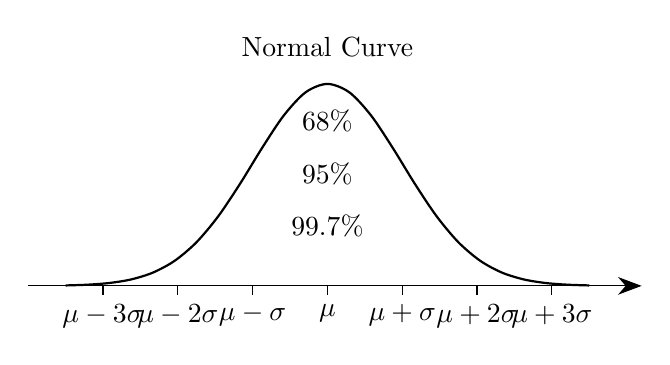
\begin{tikzpicture}[scale=0.95]
    \draw[thick, domain=-3.5:3.5, smooth, variable=\x] plot (\x,{2.7*exp(-\x*\x/2)});
    \draw[-{Stealth[length=3mm]}] (-4,0) -- (4.2,0);
    \foreach \x/\label in {-3/$\mu-3\sigma$,-2/$\mu-2\sigma$,-1/$\mu-\sigma$,0/$\mu$,1/$\mu+\sigma$,2/$\mu+2\sigma$,3/$\mu+3\sigma$}
    {
        \draw (\x,0) -- (\x,-0.12) node[below] {\label};
    }
    \node at (0,3.2) {Normal Curve};
    \node at (0,2.2) {$68\%$};
    \node at (0,1.5) {$95\%$};
    \node at (0,0.8) {$99.7\%$};
\end{tikzpicture}
\end{center}

For a \textbf{normal distribution}: about $68\%$ of the data lie within $1$ standard deviation of the mean, about $95\%$ lie within $2$ standard deviations, and about $99.7\%$ lie within $3$ standard deviations.

\section{Part I: Empirical Rule}

\begin{enumerate}[leftmargin=*, label=\textbf{\arabic*.}]

\item A test has a mean score of $70$ and a standard deviation of $10$.
\begin{enumerate}[label=(\alph*)]
    \item What percent of students scored between $60$ and $80$? \answerline
    \item What percent scored between $50$ and $90$? \answerline
    \item What percent scored below $50$? \answerline
    \item What percent scored above $90$? \answerline
\end{enumerate}

\item The heights of a group of students are normally distributed with mean $64$ inches and standard deviation $3$ inches.
\begin{enumerate}[label=(\alph*)]
    \item What percent are taller than $67$ inches? \answerline
    \item What percent are shorter than $58$ inches? \answerline
    \item What percent are between $61$ and $70$ inches? \answerline
\end{enumerate}

\item A factory produces lightbulbs with a mean lifetime of $1000$ hours and a standard deviation of $100$ hours.
\begin{enumerate}[label=(\alph*)]
    \item What percent last between $900$ and $1100$ hours? \answerline
    \item If $2000$ bulbs are produced, about how many last between $800$ and $1200$ hours? \answerline
    \item About how many last more than $1100$ hours? \answerline
\end{enumerate}

\end{enumerate}

\section{Part II: Percentages, Probability, and Counts}

\begin{enumerate}[leftmargin=*, label=\textbf{\arabic*.}, start=4]

\item SAT scores are normally distributed with mean $1050$ and standard deviation $150$.
\begin{enumerate}[label=(\alph*)]
    \item What is the probability that a randomly selected student scores above $1200$? \answerline
    \item What is the probability that a randomly selected student scores below $900$? \answerline
    \item What is the probability that a randomly selected student scores between $900$ and $1200$? \answerline
\end{enumerate}

\item A shipment contains $500$ items with weights normally distributed with mean $50$ kg and standard deviation $5$ kg.
\begin{enumerate}[label=(\alph*)]
    \item What percent weigh more than $60$ kg? \answerline
    \item About how many items is this? \answerline
    \item What percent weigh between $45$ kg and $55$ kg? \answerline
\end{enumerate}

\item IQ scores are normally distributed with mean $100$ and standard deviation $15$.
\begin{enumerate}[label=(\alph*)]
    \item What percent of people have an IQ above $130$? \answerline
    \item What percent fall between $85$ and $115$? \answerline
    \item Out of $10{,}000$ people, about how many have an IQ below $70$? \answerline
\end{enumerate}

\item A cereal company fills boxes of granola bars. The box weights are normally distributed with mean $18$ ounces and standard deviation $0.5$ ounce.
\begin{enumerate}[label=(\alph*)]
    \item What is the probability that a randomly selected box weighs less than $17.5$ ounces? \answerline
    \item What is the probability that a randomly selected box weighs between $17$ and $19$ ounces? \answerline
    \item If $12{,}000$ boxes are produced, about how many weigh more than $19$ ounces? \answerline
\end{enumerate}

\end{enumerate}

\section{Part III: Finding Scores from Percentages}

\begin{enumerate}[leftmargin=*, label=\textbf{\arabic*.}, start=8]

\item A distribution has mean $80$ and standard deviation $8$.
\begin{enumerate}[label=(\alph*)]
    \item Find the interval that contains the middle $68\%$ of the data. \answerline
    \item Find the interval that contains the middle $95\%$ of the data. \answerline
\end{enumerate}

\item A normal distribution has mean $100$ and standard deviation $20$.
\begin{enumerate}[label=(\alph*)]
    \item Find the interval that contains the middle $40\%$ of the data. \answerline
    \item Find the cutoff score for the highest $5\%$. \answerline
    \item Find the cutoff score for the lowest $5\%$. \answerline
\end{enumerate}

\item Test scores are normally distributed with mean $75$ and standard deviation $5$.
\begin{enumerate}[label=(\alph*)]
    \item What score separates the top $16\%$ from the rest? \answerline
    \item What is the lowest score in the top $2.5\%$? \answerline
    \item What is the highest score in the bottom $2.5\%$? \answerline
\end{enumerate}

\item A standardized exam has mean $500$ and standard deviation $100$.
\begin{enumerate}[label=(\alph*)]
    \item Find the scores that bound the middle $95\%$ of test takers. \answerline
    \item Find the least score needed to be in the top $0.15\%$ of test takers. \answerline
    \item Find the greatest score still in the bottom $16\%$ of test takers. \answerline
\end{enumerate}

\end{enumerate}

\section{Part IV: Skewness and Mean, Median, Mode}

\begin{enumerate}[leftmargin=*, label=\textbf{\arabic*.}, start=12]

\item Complete each statement.
\begin{enumerate}[label=(\alph*)]
    \item A distribution with a tail extending to the right is \blank{1.5in} skewed, and its center measures usually follow the order \blank{2in}. \answerline
    \item A distribution with a tail extending to the left is \blank{1.5in} skewed, and its center measures usually follow the order \blank{2in}. \answerline
    \item In a perfectly symmetric distribution, the mean, median, and mode are \blank{2in}. \answerline
\end{enumerate}

\item A dataset has mean $50$, median $45$, and mode $40$.
\begin{enumerate}[label=(\alph*)]
    \item Is the distribution left-skewed, right-skewed, or symmetric? \answerline
    \item Explain your reasoning using the relative positions of the mean, median, and mode. \biganswer
\end{enumerate}

\item A dataset has mean $<$ median $<$ mode.
\begin{enumerate}[label=(\alph*)]
    \item What type of skew does this indicate? \answerline
    \item Sketch a rough graph of the distribution below.
\end{enumerate}

\vspace{0.5em}
\begin{center}
\begin{tikzpicture}[scale=0.95]
    \draw[-{Stealth[length=3mm]}] (-4,0) -- (4.2,0);
    \draw[dashed] (0,-0.4) rectangle (0,2.6);
\end{tikzpicture}
\end{center}

\item For each description, state whether the distribution is \textbf{left-skewed}, \textbf{right-skewed}, or \textbf{symmetric}.
\begin{enumerate}[label=(\alph*)]
    \item Most families have moderate incomes, but a few have extremely high incomes. \answerline
    \item Most students score near the middle on a test, with about the same shape on both sides. \answerline
    \item Most people finish a short online survey quickly, but a few take much longer. \answerline
\end{enumerate}

\end{enumerate}

\section{Part V: Comparing Distributions Graphically}

Use the descriptions below to answer the questions.

\begin{enumerate}[leftmargin=*, label=\textbf{\arabic*.}, start=16]

\item Distribution A is bell-shaped and centered at $50$. Distribution B is bell-shaped and centered at $70$. The two curves have the same spread.
\begin{enumerate}[label=(\alph*)]
    \item Which distribution has the higher mean? \answerline
    \item Which distribution has the higher standard deviation? \answerline
    \item Explain how you know. \biganswer
\end{enumerate}

\item Distribution A and Distribution B have the same mean. Distribution A is narrow and steep, while Distribution B is wider and flatter.
\begin{enumerate}[label=(\alph*)]
    \item Which distribution has the larger standard deviation? \answerline
    \item Which distribution has more variability? \answerline
    \item Which distribution is more likely to produce values far from the mean? Explain. \biganswer
\end{enumerate}

\item Two classes took different versions of an exam. The score distributions are both approximately normal. Class X has a distribution centered at $82$ with standard deviation $4$. Class Y has a distribution centered at $82$ with standard deviation $9$.
\begin{enumerate}[label=(\alph*)]
    \item Which class has the greater mean score? \answerline
    \item Which class has the greater spread? \answerline
    \item In which class would you expect more scores to be very high or very low? Why? \biganswer
\end{enumerate}

\end{enumerate}

\section{Part VI: Comparing Distributions with Z-Scores}

Use the z-score formula when needed:
\[
z = \frac{x-\mu}{\sigma}
\]

\begin{enumerate}[leftmargin=*, label=\textbf{\arabic*.}, start=19]

\item Student A scores $85$ on a test with mean $75$ and standard deviation $5$. Student B scores $90$ on a test with mean $80$ and standard deviation $10$.
\begin{enumerate}[label=(\alph*)]
    \item Find each student's z-score. \answerline
    \item Who performed better relative to their group? \answerline
\end{enumerate}

\item A basketball player scores $20$ points in a game.
\begin{itemize}
    \item League 1: mean $15$, standard deviation $5$
    \item League 2: mean $10$, standard deviation $2$
\end{itemize}
\begin{enumerate}[label=(\alph*)]
    \item Compute the z-score of $20$ points in each league. \answerline
    \item In which league is that performance more impressive relative to the rest of the league? \answerline
\end{enumerate}

\item A company evaluates employee productivity.
\begin{itemize}
    \item Department A: mean $100$, standard deviation $10$
    \item Department B: mean $80$, standard deviation $5$
\end{itemize}
One employee scores $110$ in Department A and another scores $90$ in Department B.
\begin{enumerate}[label=(\alph*)]
    \item Find both z-scores. \answerline
    \item Who is performing better relative to their department? \answerline
    \item Use the empirical rule to estimate the percentile rank of each employee. \biganswer
\end{enumerate}

\item A runner completes a race in $54$ minutes. In Race A, the mean time is $60$ minutes with standard deviation $3$ minutes. In Race B, the mean time is $70$ minutes with standard deviation $8$ minutes.
\begin{enumerate}[label=(\alph*)]
    \item Find the runner's z-score for each race. \answerline
    \item In which race was the runner's performance better relative to the field? Explain. \biganswer
\end{enumerate}

\end{enumerate}

\section{Part VII: Challenge Problems}

\begin{enumerate}[leftmargin=*, label=\textbf{\arabic*.}, start=23]

\item A normal distribution has mean $60$ and standard deviation $6$.
\begin{enumerate}[label=(\alph*)]
    \item What percent of the values lie between $48$ and $72$? \answerline
    \item If there are $1200$ values, about how many fall outside this range? \answerline
\end{enumerate}

\item A normal distribution has $2.5\%$ of its values above $90$.
\begin{enumerate}[label=(\alph*)]
    \item Approximately how many standard deviations above the mean is $90$? \answerline
    \item If the standard deviation is $7$, what is the mean? \answerline
\end{enumerate}

\item A school plans to give awards to the top $10\%$ of students.
The exam scores are normally distributed with mean $70$ and standard deviation $8$.
\begin{enumerate}[label=(\alph*)]
    \item Estimate the cutoff score for an award. \answerline
    \item If $300$ students took the exam, about how many receive awards? \answerline
\end{enumerate}

\item A company manufactures metal rods with lengths normally distributed with mean $100$ cm and standard deviation $2$ cm.
\begin{enumerate}[label=(\alph*)]
    \item What is the probability that a rod is between $98$ cm and $102$ cm long? \answerline
    \item What is the probability that a rod is shorter than $96$ cm? \answerline
    \item If $5000$ rods are produced, about how many are longer than $104$ cm? \answerline
\end{enumerate}

\end{enumerate}

\section{Optional Extension: Quick Visual Comparison Prompts}

For each pair of distributions below, state which one has the \textbf{greater mean} and which one has the \textbf{greater standard deviation}.

\begin{enumerate}[leftmargin=*, label=\textbf{\Alph*.}]
    \item Distribution 1 is centered farther to the right than Distribution 2, but both have the same width.
    \biganswer
    \item Distribution 1 and Distribution 2 have the same center, but Distribution 2 is much wider.
    \biganswer
    \item Distribution 1 is farther right and also wider than Distribution 2.
    \biganswer
\end{enumerate}

\end{document}
